\chapter{Conceitos básicos}

\section{Definição de rastreamento}

Segundo Lepetit e Fua \cite{lepetit}, rastrear um objeto é identificar sua posição e orientação na cena quando o objeto e/ou a câmera estão em movimento. Em outras palavras, é saber a posição e orientação da câmera virtual (ou pose da câmera) em relação ao objeto presente na cena, dada uma entrada de imagem ou vídeo.

\section{Representação da câmera}

Neste trabalho de graduação será usado um modelo tradicional de câmera com orifício para representar a câmera virtual. A projeção 2D é formada a partir de dados 3D seguindo um modelo de projeção em perspectiva. A formação da imagem pode então ser definida como a projeção de pontos do espaço 3D para um plano 2D. Seja $M = [X, Y, Z]^T$ um ponto 3D em coordenadas de mundo e $m = [u, v]^T$ um ponto 2D em coordenadas de tela, eles se relacionam de acordo com a equação

\begin{equation}
\label{projection_eq}
s\tilde{m} = P\tilde{M}
\end{equation}

em que $s$ é um fator de escala que indica a resolução em que o modelo será projetado na tela, $\tilde{m} = [u, v, 1]^T$ e $\tilde{M} = [X, Y, Z, 1]^T$ são os pontos $m$ e $M$ em coordenadas homogêneas, e $P$ é uma matriz de projeção em perspectiva $3 \times 4$. A matriz $P$ contém informações da câmera como parâmetros de calibração, posição da câmera no espaço 3D e orientação da câmera. Ela pode ser decomposta da seguinte forma:

\begin{equation}
\label{matrix_p}
P = K[R | t]
\end{equation}

Em \eqref{matrix_p}, $K$ representa os parâmetros intrínsecos da câmera. Esses parâmetros, na maioria dos experimentos, não mudam no decorrer do rastreamento e são conhecidos previamente através de uma calibração da câmera. O parâmetro $K$ também é conhecido como matriz de calibração da câmera \cite{lepetit} e contém informações como fator de escala, distância focal e o ponto de interseção do eixo óptico da câmera e o plano de projeção. O que foi discutido até agora pode ser observado na \figref{projection_scheme}.

\begin{figure}[!ht]
\centering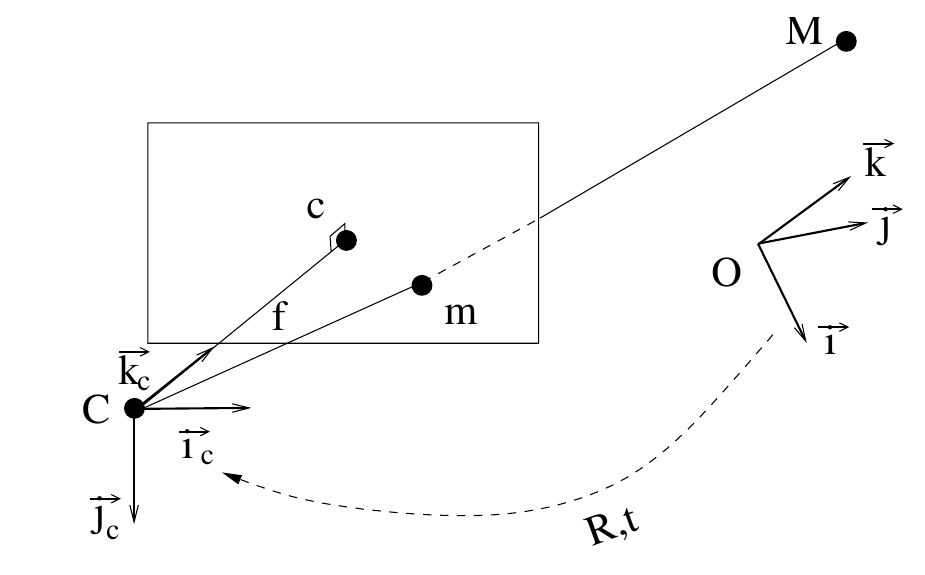
\includegraphics[width=5in]{monografia/projection_scheme.png}
\caption{Esquema de projeção em perspectiva. Observe na imagem que $(\mathbf{O}, \vec{i}, \vec{j}, \vec{k})$ é o sistema de coordenadas do mundo, $(\mathbf{C}, \vec{i_c}, \vec{j_c}, \vec{k_c})$ é o sistema de coordenadas da câmera, $\mathbf{M}$ é um ponto 3D e $\mathbf{m}$ é sua projeção 2D no plano. Retirado de \cite{lepetit}.}
\label{projection_scheme}
\end{figure}

Ainda na equação \eqref{matrix_p}, $[R | t]$ é uma matriz $3 \times 4$ e representa os parâmetros extrínsicos da câmera. Diferente dos parâmetros intrínsecos, os extrínsicos mudam no decorrer do rastreamento.

Ao observar a equação \eqref{projection_eq} pode-se dizer que tendo um ponto 2D $\tilde{m}$ da imagem e um fator de escala $s$ (que também é conhecido), para que o ponto $\tilde{M}$ seja projetado em $\tilde{m}$ é necessário descobrir a matriz $P$ da câmera que realize essa operação, ou seja, um $P$ que torne $P\tilde{M_i} \equiv \tilde{m_i}$ válido para todo $i$. Como foi visto em \eqref{matrix_p}, $K$ é um parâmetro conhecido da câmera, então o que queremos saber, na verdade, é a matriz $[R | t]$, que daqui para frente será chamada de \emph{pose da câmera}.

\subsection{Cálculo da pose}

O cálculo da pose é na verdade uma estimativa para que o ponto $\tilde{M_i}$, ao ser projetado em coordenadas de tela ($P\tilde{M_i}$), seja o mais próximo possível do ponto $m_i$, que é um ponto 2D extraído da imagem. A distância do ponto projetado $P\tilde{M_i}$ para seu correspondente extraído da imagem ($m_i$) é chamada de erro de reprojeção. O objetivo das técnicas de rastreamento que usam essa representação de câmera é encontrar uma pose ($[R | t]$) cuja soma dos erros de reprojeção seja a menor possível. Em outras palavras, deseja-se resolver a equação

\begin{equation}
[R | t] = \argmin_{[R | t]} \sum_i \text{dist}^2(P\tilde{M_i}, m_i)
\end{equation}

Essa equação não fornece uma solução polinomial de forma fechada, por isso métodos de otimização como o Gauss-Newton ou o Levenberg–Marquardt devem ser utilizados.

Estimadores robustos como um \emph{M-estimator} também podem servir, e são bastante úteis. O papel principal destes estimadores é eliminar a influência de \emph{outliers}, que são algumas poucas correspondências 2D-3D grosseiramente erradas, mas que podem influenciar bastante no resultado final.

\section{Rastreamento}

Para auxiliar no cálculo da pose é preciso extrair \emph{features}, que são componentes mais simples da cena como marcadores \cite{ref_marcadores}, arestas do objeto \cite{ref_arestas}, textura do objeto \cite{ref_textura}, pontos de interesse \cite{ref_pontosdeinteresse}: qualquer coisa que sirva para recuperar a pose (3D) da câmera virtual a partir de uma sequência de imagens 2D. Conhecendo a posição 3D dessas \emph{features} no quadro anterior e extraindo sua posição 2D no quadro atual já é um grande passo para realizar o rastreamento. A intenção dos algoritmos de rastreamento é descobrir uma pose da câmera que, ao usá-la para fazer a projeção 2D destas \emph{features} 3D, essas \emph{features} tenham as mesmas posições 2D das que foram extraídas do quadro atual.

Como foi dito anteriormente, existe na literatura vários tipos de informações que podem ser usadas como \emph{features}. Uma das formas mais conhecidas de rastreamento é a que insere marcadores externos na cena, como o da \figref{marcador_modelo}. Nesta técnica deve-se conhecer a priori o marcador a ser utilizado. O trabalho consiste então em encontrar o marcador em cada quadro e saber que operação feita na câmera (rotação, translação ou cisalhamento) deixaria o marcador tomado como modelo (\figref{marcador_modelo}) com a mesma configuração que o marcador extraído da imagem (\figref{marcador_extraido}).

\begin{figure}[!ht]
	\centerline{
		\subfloat[Exemplo de marcador externo]{
			
\includegraphics[width=0.25\textwidth]{monografia/pattSample1}
			\label{marcador_modelo}
		}
		\hfil
		\subfloat[Exemplo de marcador extraído de uma imagem]{
			\begin{tikzpicture}
				\pgftext[at=\pgfpointorigin]{
					\pgflowlevel{\pgftransformcm{1}{0.7}{0}{1}{\pgfpoint{0}{0}}}
					% \pgfdeclareimage[height=0.2\textwidth]{deformedtag}{monografia/pattSample1} % on preample
					% \pgfuseimage{deformedtag}
					
\includegraphics[height=1in]{monografia/pattSample1}
				}
			\end{tikzpicture}
			\label{marcador_extraido}
		}
	}
	\caption{Exemplo de marcador e sua projeção}
\end{figure}

O uso de marcadores, no entanto, requer que uma interferência no ambiente seja feita e, apesar de simplificar o rastreamento 3D, nem sempre é usado. Isto acontece porque podem existir limitações técnicas que impeçam a introdução prévia de elementos auxiliares ou pode até existir limitações baseadas na decisão do usuário final. Neste caso deve-se buscar \emph{features} que estejam naturalmente na cena, o que muitas vezes é parte do próprio objeto a ser rastreado. Abrir mão de marcadores externos torna o rastreamento muito mais desafiador, e a discussão dessas técnicas será o foco do resto do trabalho.

Existem várias formas de rastrear um objeto na cena sem a utilização de marcadores externos \cite{teichrieb2007survey} e entre elas existe o rastreamento baseado em modelo e o \emph{Structure from Motion} (\emph{SfM}).

O rastreamento baseado em modelo é caracterizado pelo uso de um modelo 3D pré-definido do objeto a ser rastreado. O modelo serve para saber as características do objeto que serão usadas para rastrear. Já na técnica baseada em \emph{Structure from Motion} (\emph{SfM}) \cite{teichrieb2007survey} não é necessário um conhecimento prévio da cena e, por isso, é bastante útil quando o ambiente a ser rastreado é desconhecido.

Ao se comparar as duas técnicas pode-se dizer que a baseada em modelos é mais eficiente que a \emph{SfM} \cite{drummondecipolla}. A \emph{SfM} baseia-se na análise de todo o \emph{frame} da sequência de vídeo para poder identificar um movimento na câmera, e sabendo-se que poucos segundos de um vídeo pode conter bastante informação, essa análise pode se mostrar lenta. A técnica baseada em modelos, por sua vez, pode tirar proveito de um modelo já conhecido do objeto a ser rastreado. Com isso apenas características chaves precisam ser analisadas para o rastreamento.

\subsection{Rastreamento sem marcadores baseado em modelo}

Algumas das técnicas de rastreamento sem marcadores, como foi dito anteriormente, baseiam-se no uso de um modelo 3D (feito em uma ferramenta CAD como o 3D Studio Max \cite{ref_3dsmax} ou Maya \cite{ref_maya}) do objeto a ser rastreado. Ter esse modelo é importante, já que a maioria das técnicas de rastreamento sem marcadores utiliza \emph{features} do próprio objeto. Considerando uma análise superficial, a ideia é equivalente ao método que utiliza marcadores: extrair as \emph{features} da imagem 2D capturada e tentar chegar a uma pose da câmera virtual que, ao ser usada para fazer a projeção 2D do modelo 3D do objeto, chegamos a uma imagem equivalente àquela capturada do objeto.

As técnicas baseadas em modelo podem usar uma gama de informações do objeto para dar suporte ao processo de rastreamento, sendo uma delas a textura do objeto \cite{teichrieb2007survey}. O rastreamento baseado em textura pode ser feito de diferentes formas: existe uma técnica que aplica um modelo de distorção a uma imagem de referência \cite{ref_19tgchico}; outra que utiliza pontos de interesses, que se baseia no casamento de \emph{features} das imagens recuperadas com \emph{features} de uma imagem de template pré-definida \cite{lepetit}.

Além da textura do objeto, um outro tipo de informação que pode ser usada são as suas arestas. O processo de casamento de aresta pode ser descrito da seguinte forma: tendo as arestas do modelo CAD pré-definido, o objetivo é encontrar os pontos de forte gradiente da imagem para formar linhas (que serão as arestas do objeto) e então encontrar a pose que projeta as arestas do modelo 3D o mais próximo possível das arestas extraídas da imagem.

A escolha entra textura ou arestas do modelo depende do objeto a ser rastreado. A \figref{textura_aresta_textura} ilustra um objeto com textura cujas arestas não são bem definidas. Se for feita uma rotação no eixo $Z$, mostrado na imagem, dificilmente um algoritmo baseado em arestas irá percebê-la. Por outro lado, o objeto mostrado na \figref{textura_aresta_aresta}, apesar de não ter textura, tem arestas bem definidas.

\begin{figure}[!ht]
	\centerline{
		\subfloat[Este objeto, por ser cilíndrico, não possui arestas bem definidas. No entanto seu desenho é um convite ao uso de técnicas de rastreamento baseadas em textura.]{
			\shortstack{\textbf{FAZER:} Lata de coca-cola com\\um eixo Z atravessando no meio}
			\label{textura_aresta_textura}
		}
		\hfil
		\subfloat[Este objeto não possui textura, porém suas arestas são bem definidas. Imagem retirada de \cite{marchand_modelbased}.]{
			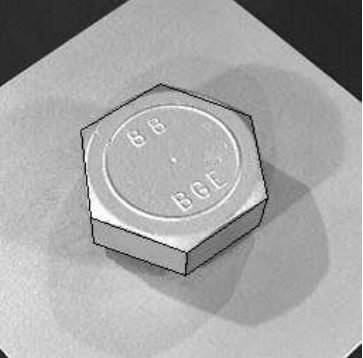
\includegraphics[width=0.25\textwidth]{monografia/textura_aresta_aresta}
			\label{textura_aresta_aresta}
		}
	}
	\caption{Dois tipos de objetos: um com textura e outro com arestas bem definidas}
\end{figure}

\subsection{Técnicas de rastreamento baseado em arestas}

Independente das técnicas que serão apresentadas abaixo, o rastreamento baseado em aresta segue praticamente o mesmo \emph{pipeline}. Primeiro é preciso saber a pose do \emph{frame} anterior. Se for o primeiro \emph{frame} este, ainda assim, terá que ser informado, e é por isso que nos experimentos é preciso ser definida uma pose inicial. Depois de obtida a pose do \emph{frame} anterior, o \emph{frame} atual é capturado a partir de uma sequência de vídeo. Essa imagem capturada será então analisada em busca de pontos de forte gradiente para a extração de bordas. Obtém-se então as arestas do modelo que estão visíveis após serem projetadas utilizando a pose do quadro anterior. As arestas visíveis são aquelas que ao serem projetadas na tela não são oclusas por outras partes do objeto (considerando um objeto opaco). Em seguida a projeção das arestas visíveis são comparadas com as bordas extraídas das imagens. Nessa comparação é feito um casamento entre a aresta 3D projetada do modelo e a aresta extraída da imagem (veja \figref{cubo_pipeline_drummond}). Esse casamento dá à aresta extraída da imagem uma estimativa inicial de sua posição 3D. Após isso é feito o cálculo da pose para que as arestas do modelo 3D projetado na tela, utilizando a pose calculada, fique o mais próximo possível das arestas extraídas da imagem. Esta pose será então a pose do \emph{frame} atual.

\begin{figure}[!ht]
\centering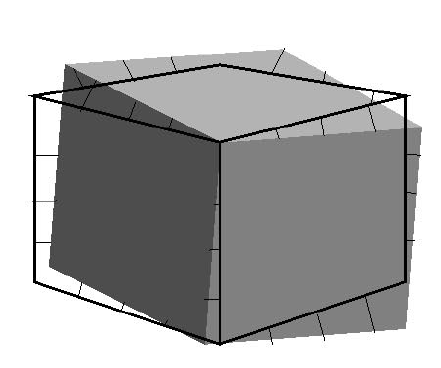
\includegraphics[width=2in]{monografia/cubo_pipeline_drummond}
\caption{Casamento de arestas do modelo (\emph{wireframe}) com arestas do objeto na imagem (cubo cinza). Imagem retirada de \cite{drummondecipolla}.}
\label{cubo_pipeline_drummond}
\end{figure}

Como descrito no \emph{pipeline} anterior, uma das etapas do rastreamento baseado em aresta é a extração das arestas do quadro atual, que é uma imagem 2D. Duas técnicas que valem a pena serem mencionadas são a extração explícita de aresta \cite{extracao_explicita} e a técnica da amostragem de pontos\cite{drummondecipolla}.

Na primeira técnica são extraídos segmentos de reta da imagem utilizando algum algoritmo de detecção de linha, como a transformada de Hough, ao mesmo tempo em que o modelo é renderizado utilizando a pose do \emph{frame} anterior, como mostra a \figref{carro_extracao_explicita}. Um procedimento recursivo é então utilizado com a finalidade de encontrar as melhores correspondências entre as arestas do modelo 3D e os segmentos de reta 2D extraídos da imagem. Neste procedimento as arestas projetadas do modelo são agrupadas com os segmentos de reta extraídos de acordo com a menor distância de Mahalanobis.

\begin{figure}[!t]
\centering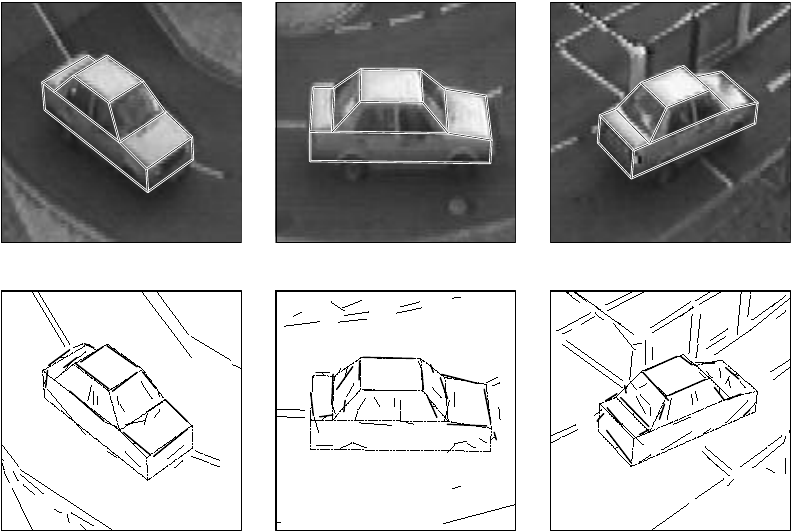
\includegraphics[width=0.9\textwidth]{monografia/carro_extracao_explicita}
\caption{Processo de extração explícita de arestas. Imagem retirada de \cite{extracao_explicita}.}
\label{carro_extracao_explicita}
\end{figure}

\section{NULL! Seção a ser reescrita}

% Uma outra técnica de rastreamento é a baseada em \emph{Structure from Motion} (\emph{SfM}) \cite{teichrieb2007survey}. Nesta abordagem não é necessário um conhecimento prévio da cena e, por isso, é bastante útil quando o ambiente a ser rastreado é desconhecido. Apesar disso, a \emph{SfM} tem a desvantagem de ser bastante complexa e não tão eficiente para rastrear uma sequência em vídeo. Isso se deve ao fato de um vídeo conter bastante informação, e muitas vezes apenas uma pequena parte disso seria suficiente para rastrear o movimento da câmera \cite{drummondecipolla}. É nesse aspecto que o rastreamento baseado em modelos se destaca, pois são observados apenas pontos chaves da cena (como os contornos do modelo, por exemplo).

\section{Rastreamento por arestas}

%Para a extração das arestas da imagem geralmente são utilizados algoritmos de detecção de borda, como o filtro Sobel.

% A vantagem dessa técnica é que arestas são relativamente mais fáceis de serem encontradas em uma imagem. Algoritmos para detecção de bordas são abundantes na literatura e já vem sido bastante estudado em processamento de imagens.%citation

\subsection{Técnicas}

Uma das formas de fazer o casamento entre as arestas do modelo e as arestas da imagem é usar o que pode ser chamado de extração explícita das arestas. Utilizando algum algoritmo de detecção de linha, como a transformada de Hough, as arestas da imagem são extraídas para depois serem comparadas com as do modelo na pose anterior. %cite (Hough) [3] em VTetal

% [como funciona?]. Entretanto um dos problemas desse método é a possibilidade de parte de uma aresta visível estar oculta [como mostra a figura, retirada de \cite{drummondecipolla}]. Isso pode ser interpretado pelo algoritmo como duas arestas menores e que possivelmente não vai ser casada com a aresta correspondente do modelo.

Outra forma de trabalhar com rastreamento baseado em arestas é utilizando a técnica de amostragem de pontos. Neste caso a aresta do modelo é dividida em partes iguais, chamados de amostras (ou \emph{sample-points}). Cada ponto amostrado é então comparado com pontos de forte gradiente da imagem que estão próximos da aresta. Uma das formas de fazer isso é fazer uma busca na direção normal da aresta que passa pelo ponto amostrado. O primeiro ponto de forte gradiente encontrado pode então ser considerado correspondente ao ponto amostrado. Ou seja, é possivelmente onde aquele ponto da pose anterior está no \emph{frame} atual.

% que serão utilizados para casar com as amostras extraídas da imagem.

Em outras palavras o casamento das amostras do modelo com os pontos extraídos da imagem acontece da seguinte forma: primeiro o modelo do \emph{frame} anterior é renderizado a fim de ter uma estimativa inicial da posição do objeto no frame atual; Para cada aresta do modelo são extraídos $N$ amostras que posteriormente serão comparadas com a imagem obtida do frame atual; Em cada amostra do modelo é feita uma busca na normal da aresta a fim de encontrar pontos de forte gradiente (bordas), o que podemos supor que são pontos da aresta da imagem. A partir do casamento das amostras do modelo com os pontos de forte gradientes da imagem, pode ser feita uma estimativa do movimento da câmera.

A extração explícita das arestas tem a vantagem de ser mais robusta, porém é restrita apenas a objetos poligonais. A amostragem de pontos, por sua vez, mostra-se bastante útil quando as arestas não são formadas por retas. Há também a vantagem de trabalhar melhor com arestas oclusas, como mostra a \figref{occlusion}.

\begin{figure}[ht!]
\centering
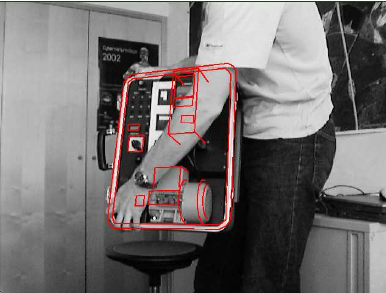
\includegraphics{monografia/occlusion.png}
\caption{Objeto com oclusão parcial das arestas. Imagem retirada de \cite{wuest}}
\label{occlusion}
\end{figure}

Na primeira técnica a aresta parcialmente oclusa seria considerada duas arestas diferentes, enquanto que a amostragem de pontos seria capar de identificá-la como uma aresta só.

\begin{comment}
\subsection{Trabalhando com múltiplas hipóteses}

Algo comum de acontecer na etapa de casamento das amostras do modelo com os pontos de forte gradiente da imagem é que, ao percorrer a normal para achar pontos de forte gradiente, a busca pode retornar mais de um resultado. Ou seja, é possível haver mais de uma hipótese de pontos da imagem para serem casados com uma amostra do modelo. [isso parece ser muito específico]

\subsection{Rascunho}

extração explícita de arestas (ruim por causa da oclusão \cite{drummondecipolla}) \\
amostragem de pontos (sample points. a que eu uso) \\

renderizar o modelo, localizar as arestas visiveis do modelo. a partir dela, extrair sample points. tentar fazer um match das arestas do modelo com as arestas da imagem obtida\cite{drummondecipolla} \\
explicar que pegamos uma aresta do modelo, pegamos alguns sample points. a partir dos sample points seguimos pela normal do ponto e tentamos achar os pontos de forte gradiente. podem existir vários pontos de forte gradiente para um único \emph{sample point} (múltiplas hipóteses) \\

explicar como a escolhas das múltiplas hipóteses podem ser feitas. deixar um gancho para o capítulo seguinte que explica como fazer a escolha utilizando o k-means \\

outliers happens. podem ter outras coisas que formam uma aresta. \\
\end{comment}

\begin{comment}
Em um reprodução de vídeo, rastrear um objeto se caracteriza por identificar a sua posição na cena quando tanto o objeto quanto a câmera está em movimento \cite{lepetit}.

Um vídeo contém bastante informação e é preciso extrair apenas parte dela. Por isso que é usada uma técnica \emph{feature-based}, em que o processamento das imagens é restrito à localização de pontos de forte gradiente como os contornos do objeto \cite{drummondecipolla}.

Uma das formas de efetuar um rastreamento é utilizando um técnica baseada em modelos. Nesse tipo de técnina é necessário um conhecimento prévio do que vai ser rastreado. No caso, é preciso já ter um modelo 3D do objeto a ser rastreado.

* Tipos de rastreamento: SfM, Model based

sfm pega a cena toda.
model based precisa de um modelo 3D pré-construído
    * edge based
        * amostragem de pontos (sample points. é o que eu uso)
        * extração explícita das arestas (ruim por causa da oclusão \cite{drummondecipolla})
    * texture based


model based é mais simples que sfm, mas é preciso ter um modelo de antemão \cite{teichrieb2007survey}

renderizar o modelo, localizar as arestas visiveis do modelo. a partir dela, extrair sample points. tentar fazer um match das arestas do modelo com as arestas da imagem obtida\cite{drummondecipolla}

outliers happens. podem ter outras coisas que formam uma aresta. esse é o problema que eu quero resolver.

Uma das etapas mais importantes de aplicações com realidade aumentada é o rastreamento e registro da cena \cite{teichrieb2007survey}.

Falar sobre o que é rastreamento. Etapas do rastreamento: pegar imagens da camera, identificar?
\end{comment}
